\documentclass[11pt]{article}

\usepackage{graphicx}
\usepackage{url}

\begin{document}

\begin{titlepage}
	\begin{center}
    	
\includegraphics[scale=0.10]{du.png}\par
		\begin{Huge}
			\textsc{University of Dhaka}\par
		\end{Huge}
		\begin{Large}
			Department of Computer Science and Engineering\par \vspace{1cm}
			CSE-3111 : Computer Networking Lab \\[12pt]	
			\textbf{Lab Report 1 :} Lab exercises on LAN Configuration and Troubleshooting Tools (Ping, Traceroute, ARP, Static Routing, Netstat, Ifconfig, nslookup, whois, etc.)
		\end{Large}
	\end{center}  	
	\begin{large}
		\textbf{Submitted By:\\[12pt]}
			Name : Saima Akter\\[8pt]
			Roll No : 30\\[12pt]
		\textbf{Submitted On : \\[12pt]}
			January 19, 2023\\[20pt]
		\textbf{Submitted To :\\[12pt]}
			Dr. Md. Abdur Razzaque\\[12pt]
                Md Mahmudur Rahman\\[12pt]
                Md. Ashraful Islam\\[12pt]
                Md. Fahim Arefin
	\end{large}
\end{titlepage}

\section{PING}
\subsection{Basic Usage of ping on Ubuntu}
The ping tool is very straightforward to use as we don’t really need to worry about any options. When used without any options, the command will continue to ping the destination until we kill the process.\\[12pt]
To showcase how the ping tool works on Ubuntu, we can perform a ping request to a known server.

In this example, we will use “google.com” as the destination for our device to ping. It’s an excellent website to test internet connectivity with due to its distributed servers, and it rarely goes offline.

To perform this request, we need to use “ping” followed by the destination.\\[12pt]
command Line :\\[6pt]
  Ping google.com\\[12pt]
  Output : 
  \begin{figure}[!h]
\centering
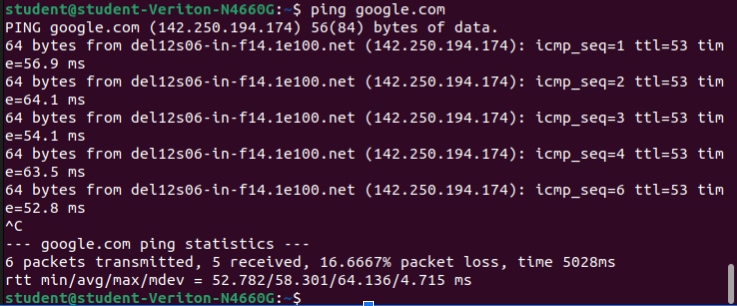
\includegraphics[width=\textwidth]{ping_google.png}
\caption{Ping google.com}
\end{figure}
\\[12pt]
command Line :\\[6pt]
  Ping 10.33.3.27\\[42pt]
  Output : 
  \begin{figure}[!h]
\centering
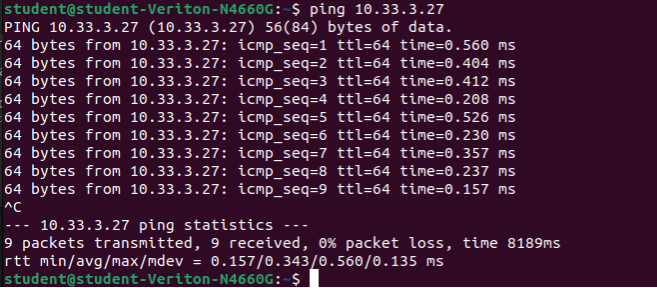
\includegraphics[width=\textwidth]{pin_ip.png}
\caption{Ping 10.33.3.27}
\end{figure}
  
\subsection{Limiting the Number of Pings}
If we want to test the network connectivity of our Ubuntu device using a limited number of pings, then there is an option we can utilize.

This option is called the “count” and can be set by using the “-c” option followed by the number of pings.\\[12pt]
command Line :\\[6pt]
  Ping -c 5 google.com    
        Output : 
  \begin{figure}[!h]
\centering
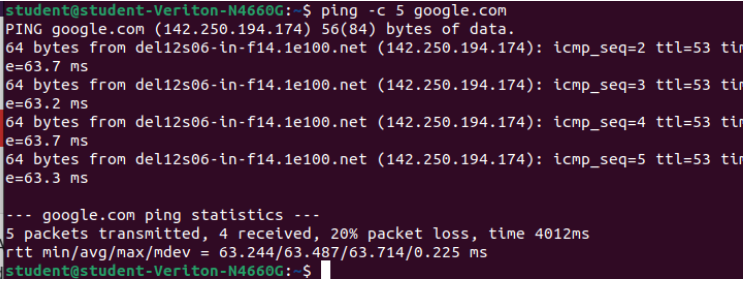
\includegraphics[width=\textwidth]{ping_count.png}
\caption{Ping -c 5 google.com}
\end{figure}

\section{TRACEROUTE}
Traceroute is a network diagnostic tool that tracks real time pathways taken by a packet on an IP network from source to destination. After, it reports the IP addresses of all the routers it pinged in between. This tool also records each hop’s time to make packets during its route to the destination.

\subsection{Run Traceroute On Ubuntu}
command Line :\\[6pt]
  traceroute google.com\\[12pt]   
        Output : 
  \begin{figure}[!h]
\centering
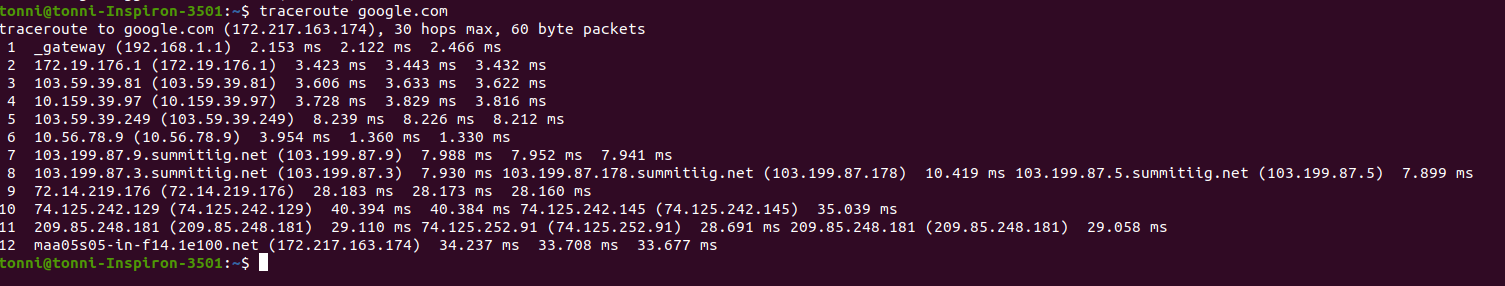
\includegraphics[width=\textwidth]{trace_google.png}
\caption{traceroute google.com}
\end{figure}
\\[12pt] 
command Line :\\[6pt]
  traceroute -d google.com\\[12pt]   
        Output : 
  \begin{figure}[!h]
\centering
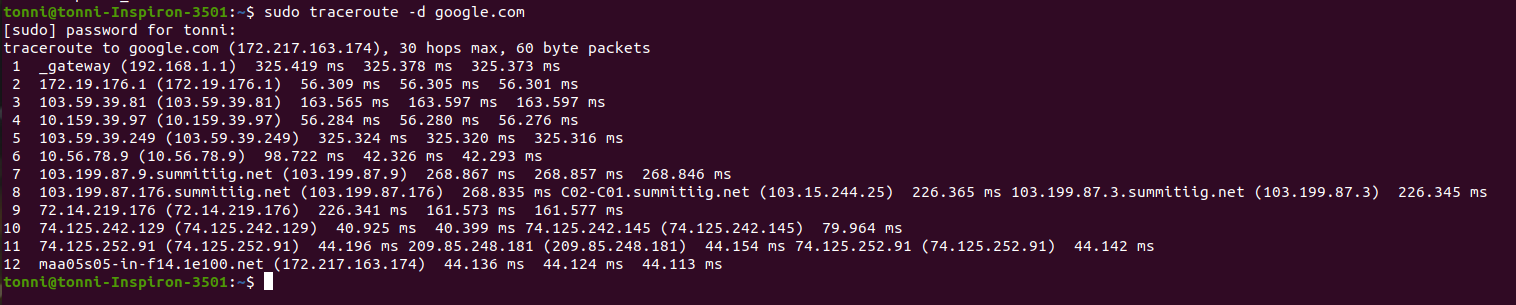
\includegraphics[width=\textwidth]{d_trace_google.png}
\caption{traceroute -d google.com}
\end{figure}

\subsection{Define Number of Probes}
By default, the Traceroute command will passed 16 probes simultaneously. we can customize the number of probes to 5 using the N option:\\[12pt]
command Line :\\[6pt]
  traceroute -N 5 google.com\\[12pt]   
        Output : 
  \begin{figure}[!h]
\centering
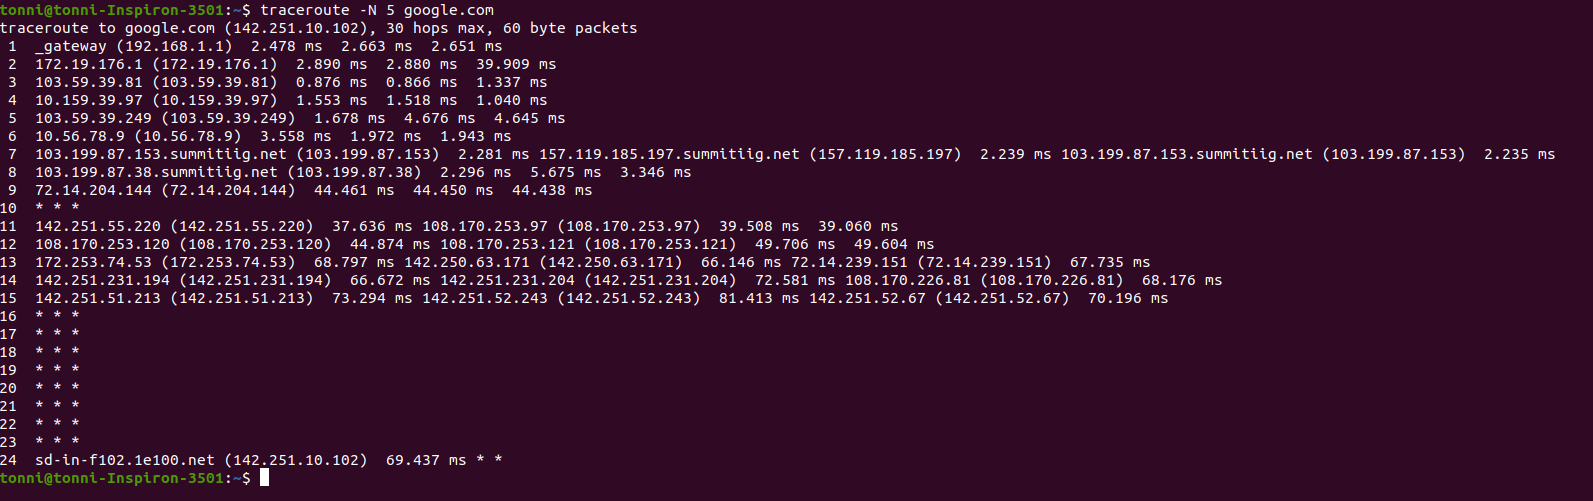
\includegraphics[width=\textwidth]{n_trace_google.png}
\caption{traceroute -N 5 google.com}
\end{figure}

\subsection{Limit the Number of Hops}
	
 By default, the Traceroute command will check the website for only 30 hops. we can set this value to 5 using the -m option:\\[12pt]
command Line :\\[6pt]
  traceroute -m 5 google.com\\[12pt]   
        Output : 
  \begin{figure}[!h]
\centering
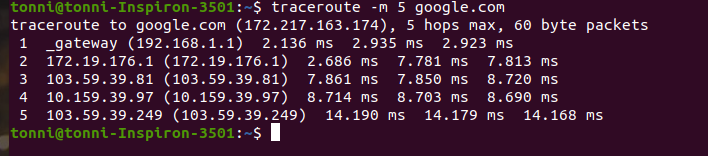
\includegraphics[width=\textwidth]{m_trace_google.png}
\caption{traceroute -m 5 google.com}
\end{figure}

\subsection{Limit the Number of Probes}
By default, the Traceroute command shows three probes at every Hop. We can change this value to 2 using the -q option:\\[12pt]
command Line :\\[6pt]
  traceroute -q 2 google.com\\[12pt]   
        Output : 
  \begin{figure}[!h]
\centering
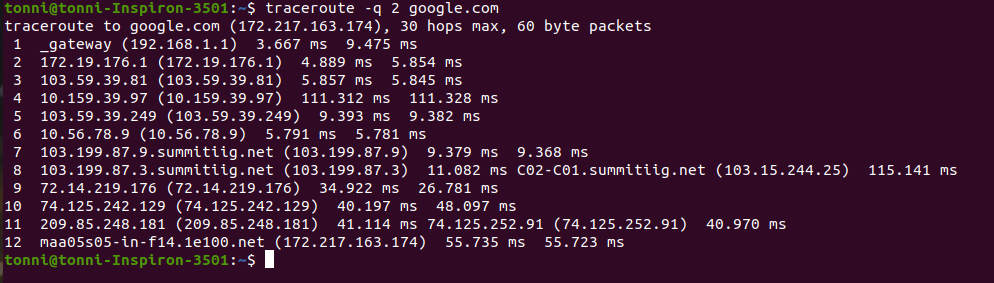
\includegraphics[width=\textwidth]{q_trace_google.png}
\caption{traceroute -q 2 google.com}
\end{figure}

\subsection{Hide Device Names}
The Traceroute command also allows us to hide the device name to make it easier to see the data. We can do it using the -n option :\\[12pt]
command Line :\\[6pt]
  traceroute -n google.com\\[12pt]   
        Output : 
  \begin{figure}[!h]
\centering
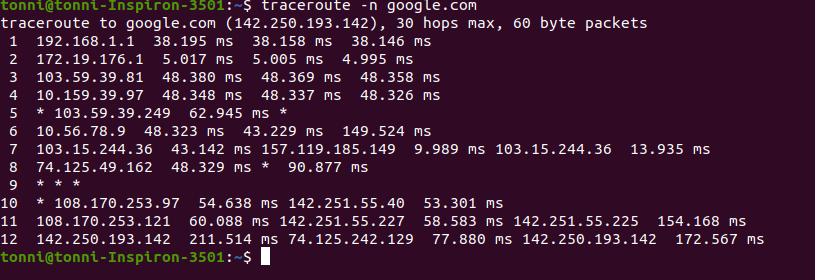
\includegraphics[width=\textwidth]{hide-trace.png}
\caption{traceroute -n google.com}
\end{figure}

\subsection{Define Initial TTL Value}
We can set the initial value of TTL to skip some hops. If we set it to five, the first test will attempt to get to hop five and skip hops one through four:\\[12pt]
command Line :\\[6pt]
  traceroute -f 15 google.com\\[12pt]   
        Output : 
  \begin{figure}[!h]
\centering
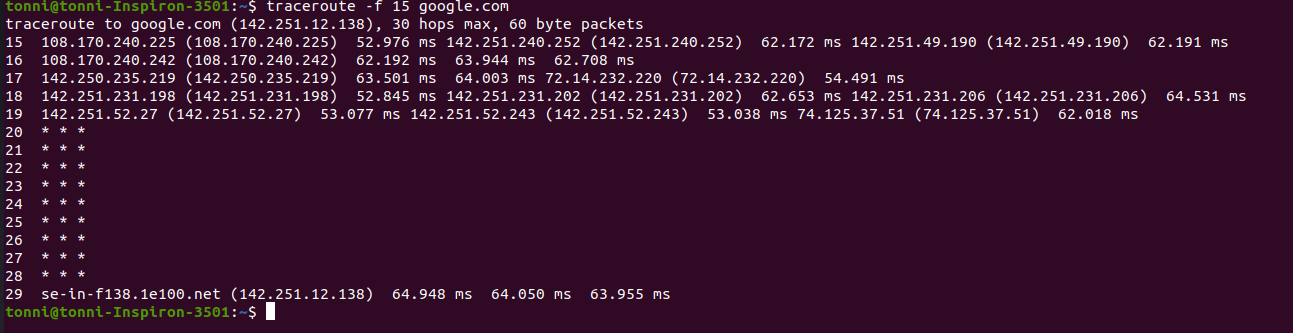
\includegraphics[width=\textwidth]{define_trace.png}
\caption{traceroute -f 15 google.com}
\end{figure}

\subsection{Increase Hope Response Rate}
We can use the -w option to increase the response rate that each Hop must wait to show the result.\\[32pt]
command Line :\\[6pt]
  traceroute -w 6.5 google.com\\[92pt]   
        Output : 
  \begin{figure}[!h]
\centering
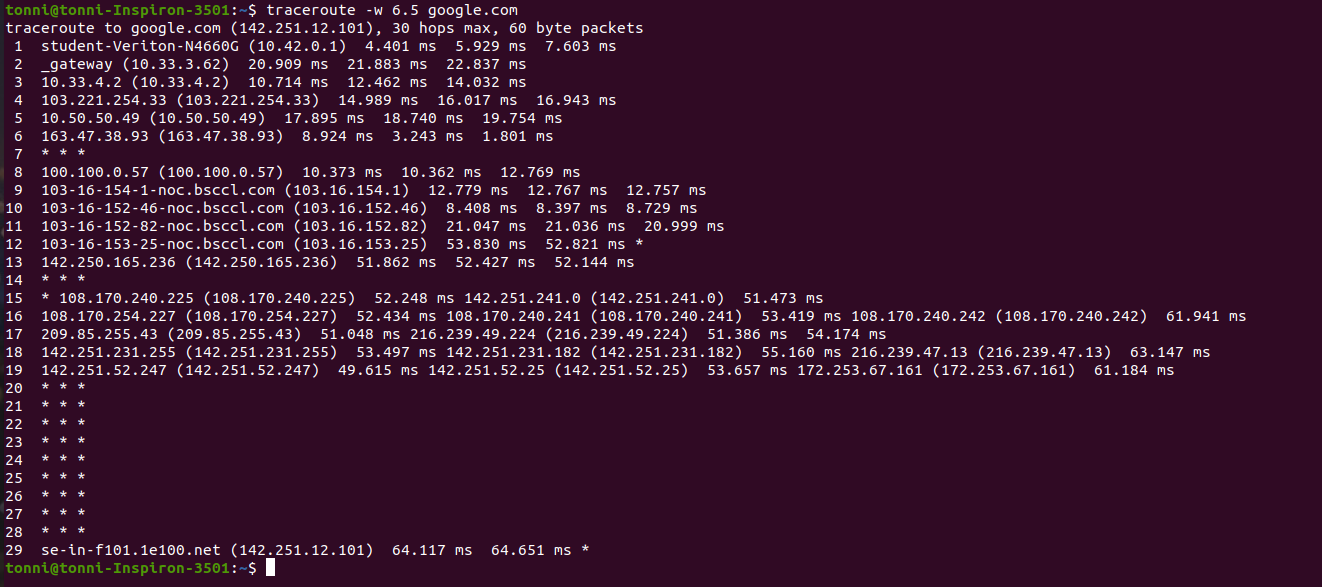
\includegraphics[width=\textwidth]{increase_trace.png}
\caption{traceroute -w 6.5 google.com}
\end{figure}

\subsection{Set Pause Time Between Probes}
The default time is 0ms. However, we can use the -z option to define our own time:\\[12pt]
command Line :\\[6pt]
  traceroute -z 0.5 google.com\\[12pt]   
        Output : 
  \begin{figure}[!h]
\centering
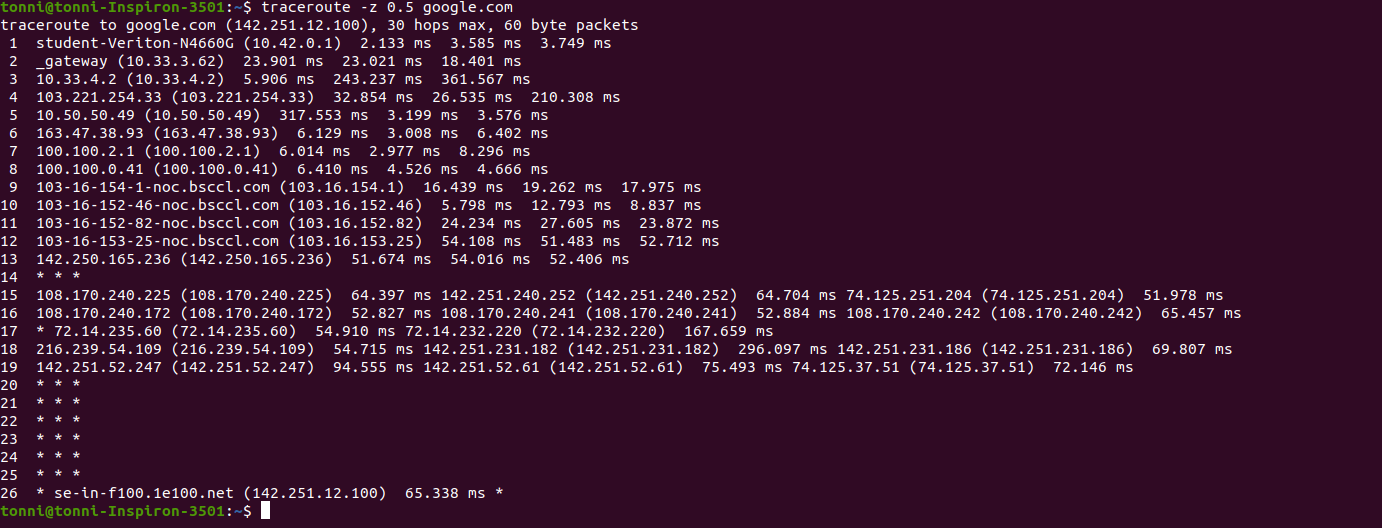
\includegraphics[width=\textwidth]{set_trace.png}
\caption{traceroute -z 0.5 google.com}
\end{figure}

\subsection{Define Specific Interface for Traceroute}
We can use the -i option to specify the interface through which traceroute should send packets. By default, the interface is selected according to the routing tab :\\[6pt]
  traceroute -i lo google.com\\[12pt]   
        Output : 
  \begin{figure}[!h]
\centering
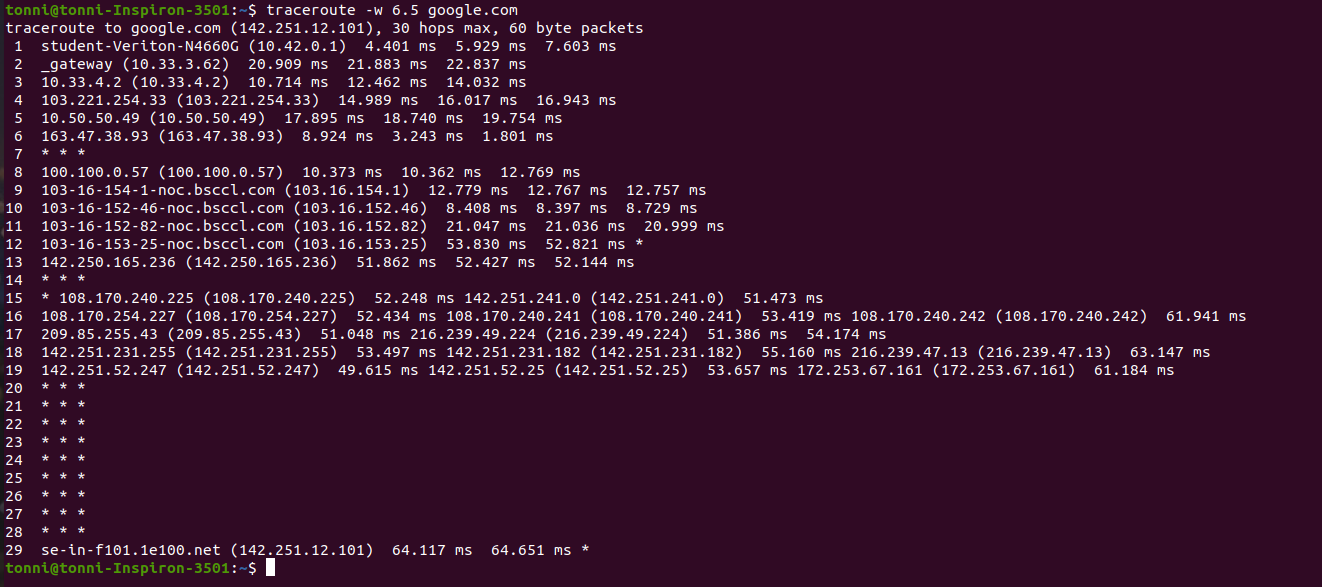
\includegraphics[width=\textwidth]{increase_trace.png}
\caption{traceroute -i lo google.com}
\end{figure}

\section{IFCONFIG}
The “ifconfig” command is used for displaying current network configuration information, setting up an ip address, netmask, or broadcast address to a network interface, creating an alias for the network interface, setting up hardware address, and enable or disable network interfaces.
\subsection{ View All Network Interface Settings}
The “ifconfig” command with no arguments will display all the active interfaces details. The ifconfig command is also used to check the assigned IP address of a server:\\[6pt]
  ifconfig\\[12pt]   
        Output : 
  \begin{figure}[!h]
\centering
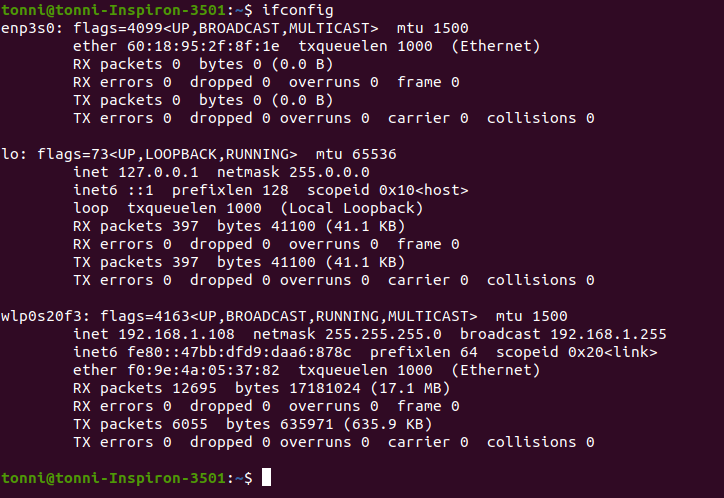
\includegraphics[width=\textwidth]{ifconfig.png}
\caption{ifconfig}
\end{figure}

\subsection{ Display Information of All Network Interfaces}
The following ifconfig command with the -a argument will display information of all active or inactive network interfaces on the server:\\[6pt]
  ifconfig -a\\[12pt]   
        Output : 
  \begin{figure}[!h]
\centering
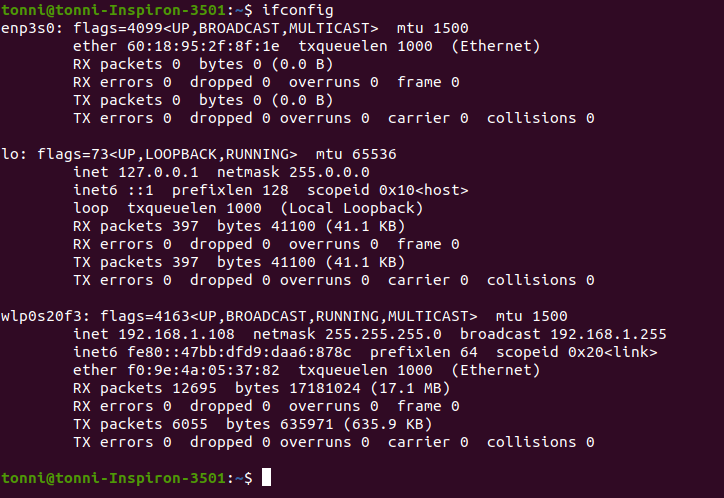
\includegraphics[width=\textwidth]{a_ifconfig.png}
\caption{ifconfig -a}
\end{figure}
\\[92pt]
\subsection{ View Network Settings of Specific Interface}
Using interface name (lo) as an argument with the “ifconfig” command will display details of the specific network interface:\\[6pt]
  ifconfig lo \\[12pt]   
        Output : 
  \begin{figure}[!h]
\centering
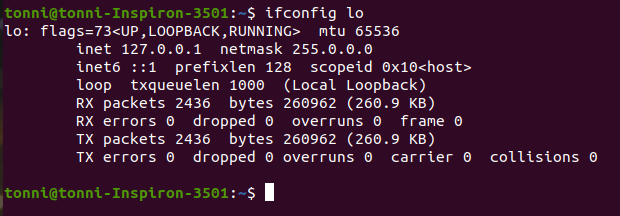
\includegraphics[width=\textwidth]{lo_ifconfig.png}
\caption{ifconfig lo}
\end{figure}
\\[72pt]
\subsection{ How to Enable a Network Interface}
The “up” or “ifup” flag with interface name (lo) activates a network interface if it is not inactive state and allowing to send and receive information\\[6pt]
  ifconfig lo up\\[12pt]   
        Output : 
  \begin{figure}[!h]
\centering
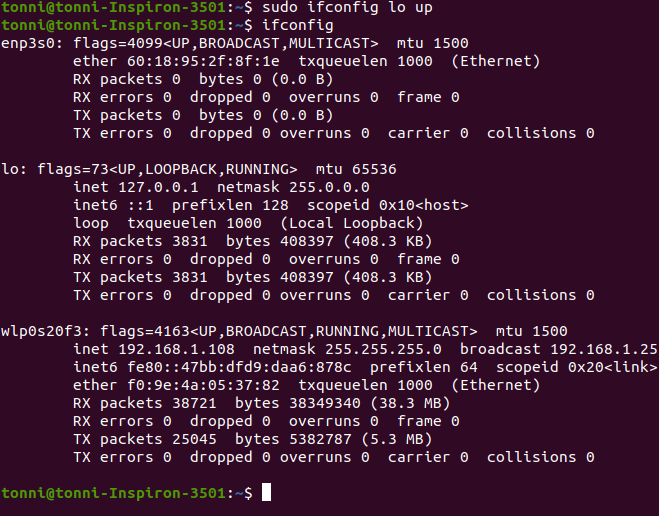
\includegraphics[width=\textwidth]{ifconfig_up.png}
\caption{ifconfig lo up}
\end{figure}

\subsection{ How to Disable a Network Interface}
The “down” or “ifdown” flag with interface name (lo) deactivates the specified network interface\\[6pt]
  ifconfig lo down\\[12pt]   
        Output : 
  \begin{figure}[!h]
\centering
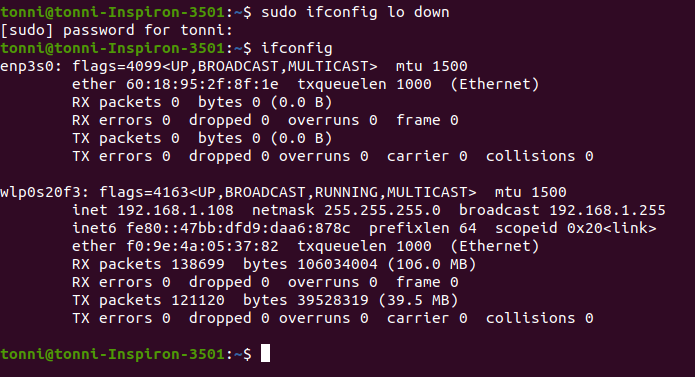
\includegraphics[width=\textwidth]{down_if.png}
\caption{ifconfig lo down}
\end{figure}
\subsection{ How to Assign an IP Address to Network Interface}
To assign an IP address to a specific interface, use the following command with an interface name (lo) and ip address that we want to set\\[6pt]
  ifconfig lo 172.16.25.125\\[12pt]   
        Output : 
  \begin{figure}[!h]
\centering
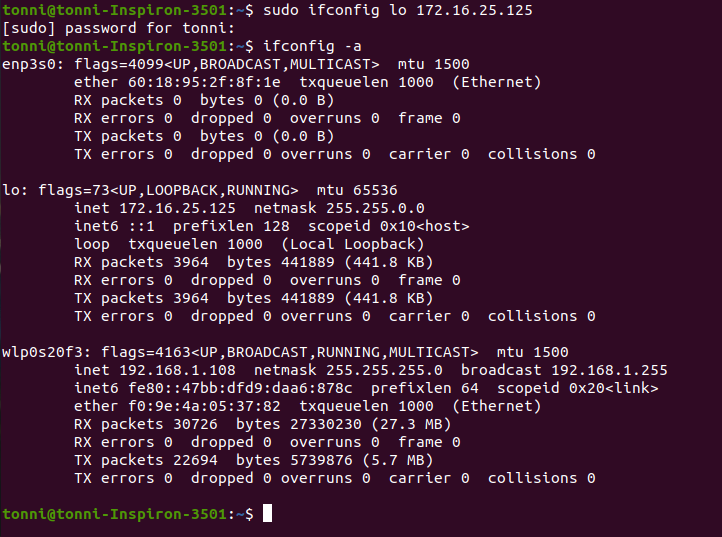
\includegraphics[width=\textwidth]{change_ip.png}
\caption{ifconfig lo 172.16.25.125}
\end{figure}
\\[42pt]
\section{ARP}
arp command manipulates the System’s ARP cache. It also allows a complete dump of the ARP cache. ARP stands for Address Resolution Protocol. The primary function of this protocol is to resolve the IP address of a system to its mac address, and hence it works between level 2(Data link layer) and level 3(Network layer). \\[12pt]
\textbf{Syntax:\\[12pt]}
arp [-v] [-i if] [-H type] -a [hostname]\\[12pt]
\textbf{Example:\\[12pt]}
  \begin{figure}[!h]
\centering
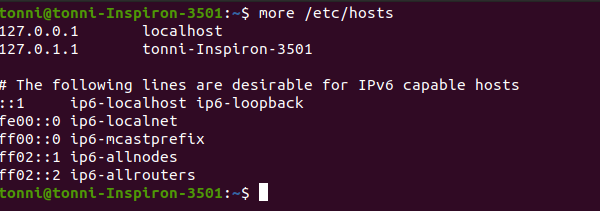
\includegraphics[width=\textwidth]{hosts.png}
\caption{Hosts}
\end{figure}
  \begin{figure}[!h]
\centering
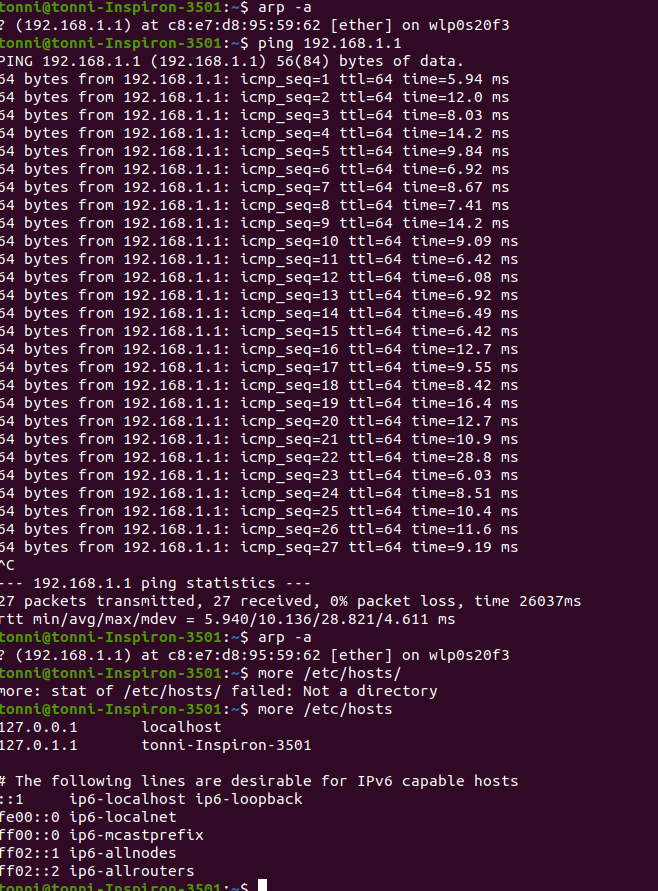
\includegraphics[width=12cm,height=10cm,keepaspectratio]{add_hosts.png}
\caption{Host add}
\end{figure}



\section{RARP}
RARP is abbreviation of Reverse Address Resolution Protocol which is a protocol based on computer networking which is employed by a client computer to request its IP address from a gateway server’s Address Resolution Protocol table or cache. The network administrator creates a table in gateway-router, which is used to map the MAC address to corresponding IP address. \\[12pt]
\textbf{Working of RARP : \\[12pt]}
The RARP is on the Network Access Layer and is employed to send data between two points in a very network. 
Each network participant has two unique addresses:- IP address (a logical address) and MAC address (the physical address). 

The IP address gets assigned by software and after that the MAC address is constructed into the hardware. 
The RARP server that responds to RARP requests, can even be any normal computer within the network. However, it must hold the data of all the MAC addresses with their assigned IP addresses. If a RARP request is received by the network, only these RARP servers can reply to it. The info packet needs to be sent on very cheap layers of the network. This implies that the packet is transferred to all the participants at the identical time. 

The client broadcasts a RARP request with an Ethernet broadcast address and with its own physical address. The server responds by informing the client its IP address.\\[12pt]
\textbf{Uses of RARP : \\[12pt]}
RARP is used to convert the Ethernet address to an IP address. It is available for the LAN technologies like FDDI, token ring LANs, etc.

\section{NSLOOKUP}
Nslookup (stands for “Name Server Lookup”) is a useful command for getting information from the DNS server. It is a network administration tool for querying the Domain Name System (DNS) to obtain domain name or IP address mapping or any other specific DNS record. It is also used to troubleshoot DNS-related problems. \\[12pt]

nslookup followed by the domain name will display the “A Record” (IP Address) of the domain. Use this command to find the address record for a domain. It queries to domain name servers and gets the details. :\\[6pt]
  nslookup google.com :\\[12pt]   
        Output : 
  \begin{figure}[!h]
\centering
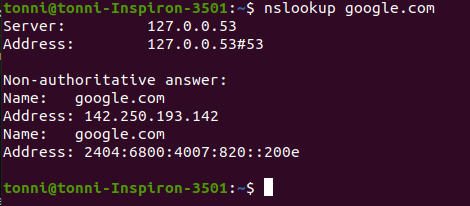
\includegraphics[width=\textwidth]{ns_1.png}
\caption{nslookup google.com :}
\end{figure}
\\[12pt]
We can also view all the available DNS records using the -type=any option. \\[6pt]
  nslookup -type=any google.com\\[12pt]   
        Output : 
  \begin{figure}[!h]
\centering
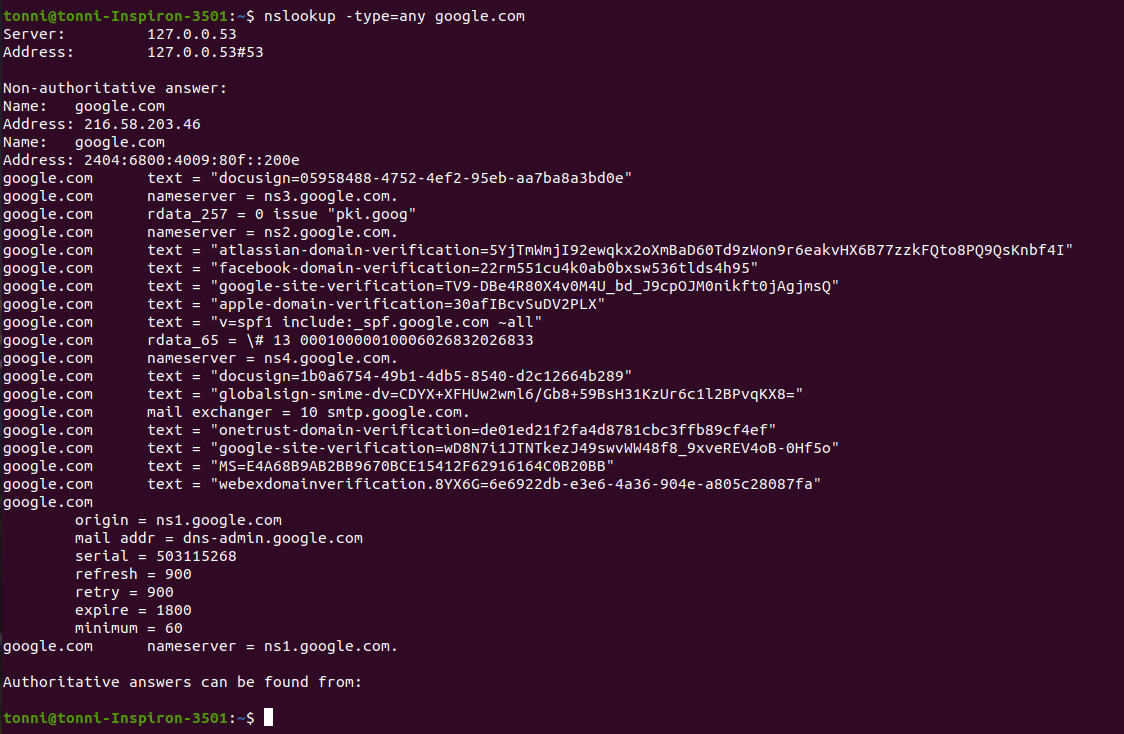
\includegraphics[width=\textwidth,height=4cm,keepaspectratio]{ns_2.png}
\caption{nslookup -type=any google.com}
\end{figure}

\section{NETSTAT}
Netstat command displays various network related information such as network connections, routing tables, interface statistics, masquerade connections, multicast memberships etc :\\[6pt]
\textbf{Example : \\[12pt]}
To show both listening and 
non-listening sockets.\\[12pt]
 netstart -a  :\\[12pt]   
        Output : 
  \begin{figure}[!h]
\centering
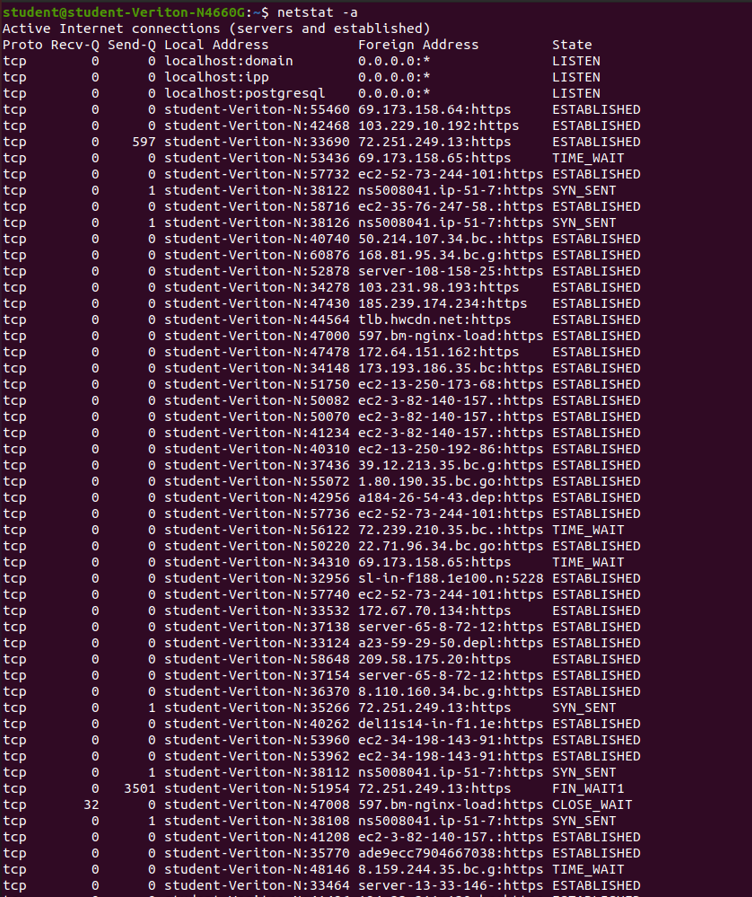
\includegraphics[width=\textwidth,height=4cm,keepaspectratio]{netstat2.png}
\caption{netstart -a :}
\end{figure}
\\[12pt]
  netstart -au\\[12pt]   
        Output : 
  \begin{figure}[!h]
\centering
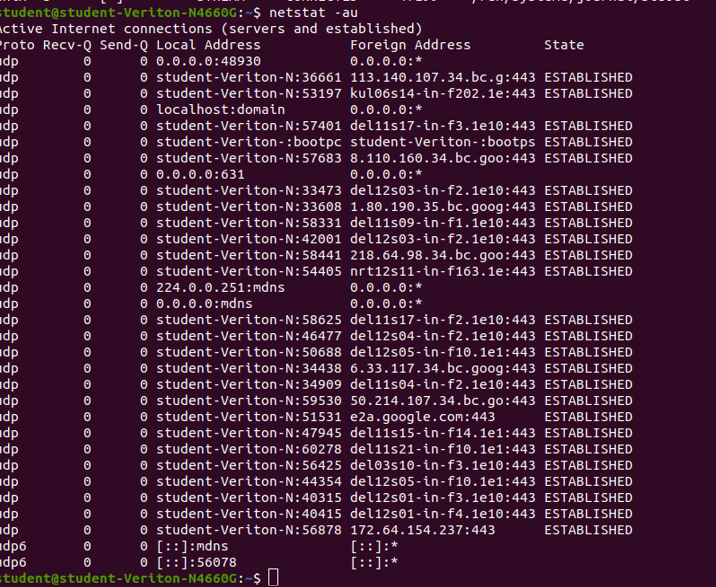
\includegraphics[width=\textwidth,height=4cm,keepaspectratio]{netstat3.png}
\caption{netstart -au}
\end{figure}
\newpage
\begin{thebibliography}{1}
\bibitem{ping}  PING : \url{https://pimylifeup.com/ubuntu-ping/#:~:text=Example%20of%20Limiting%20the%20Number%20of%20pings%20on%20Ubuntu&amp;text=To%20achieve%20this%2C%20we%20use,the%20destination%20for%20our%20pings.&amp;text=After%20running%20this%20command%2C%20your,to%20stop%20the%20process%20manually/}
\bibitem{TRACEROUTE} TRACEROUTE : \url{https://cloudinfrastructureservices.co.uk/how-to-install-traceroute-and-run-on-ubuntu-20-04/}
\bibitem{IFCONFIG} IFCONFIG : \url{https://www.tecmint.com/ifconfig-command-examples/}
\bibitem{ARPl} ARP : \url{https://www.geeksforgeeks.org/arp-command-in-linux-with-examples/}
\bibitem{RARPl} RARP : \url{https://www.geeksforgeeks.org/what-is-rarp/}
\bibitem{NSLOOKUP} NSLOOKUP : \url{https://www.geeksforgeeks.org/nslookup-command-in-linux-with-examples/}
\bibitem{NETSTAT} NETSTAT : \url{https://www.geeksforgeeks.org/netstat-command-linux/}
\end{thebibliography}

\end{document}